\item The eigenvalues of matrix \myvec{$9$ & $5$ \\ $5$ & $8$} are \hfill (CE  2012)
\begin{enumerate}
\begin{multicols}{4}
\item $-2.42$ and $6.86$
\item $3.48$ and $13.53$
\item $4.70$ and $6.86$
\item $6.86$ and $9.50$
\end{multicols}
\end{enumerate}
\item For the parallelogram $OPQR$ shown in the sketch, 
\begin{align*}
	\overrightarrow{OP}=a\hat{i}+b\hat{j} \text{ and } \overrightarrow{OR}=c\hat{i}+d\hat{j}.
\end{align*}
The area of the parallelogram is \hfill (CE  2012)
\begin{figure}[H]
    \centering
    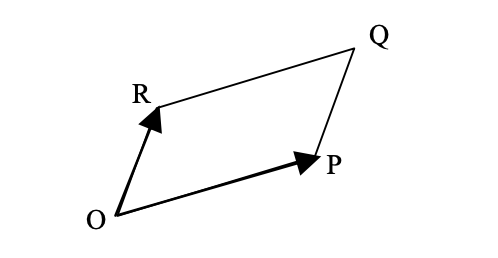
\includegraphics[width=0.3\columnwidth]{GATE/2012/CE/figs/Q29.png} 
    \caption{}
    \label{fig:placeholder-2012-ce}
\end{figure}
\begin{enumerate}
\begin{multicols}{4}
\item $a d - b c$
\item $a c + b d$
\item $a d + b c$
\item $a b - c d$
\end{multicols}
\end{enumerate}
